\documentclass{article}
\usepackage[margin=0.2in]{geometry}
\usepackage{amsmath}
\usepackage{hyperref}
\usepackage{verbatim}


\usepackage{graphicx}
\usepackage{epstopdf}

\begin{document}


\section{Rayleigh-Darcy flow}
\subsection{Governing equations}
Starting from
\begin{eqnarray}
\frac{\mu \mathbf{u}}{\Pi} &=& - \left[ \nabla p + \rho_0 g \mathbf{\hat{z}} \left(1 - \alpha (T-T_0) + \beta (C-C_0) \right) \right] \\
\frac{\partial T}{\partial t}&=&\nabla \cdot (\kappa \nabla T) \\
\nabla \cdot \mathbf{u} &=& 0
\end{eqnarray}
Based on the linear liquidus relationship, $C = C_0 - \gamma (T-T_0)$. Also define the modified pressure $P = p + \rho_0 g z$, and rewrite the first equation
\begin{eqnarray*}
\frac{\mu \mathbf{u}}{\Pi} &=& - \nabla P + \rho_0 g \mathbf{\hat{z}} (\alpha + \beta \gamma) (T-T_0) \\
&=& - \nabla P + \rho_0 g \mathbf{\hat{z}} \Gamma (T-T_0)
\end{eqnarray*}
\subsection{Non-dimensionalising, as per Worster 1997}
Define dimensionless temperature $T' = \frac{T - T_0}{T_1 - T_0} = \frac{T - T_0}{\Delta T}$ and scale the other variables with:
\begin{eqnarray*}
&&\text{Velocity: } V \\
&&\text{Length: } \frac{\kappa}{V} \\
&&\text{Time: } \frac{\kappa}{V^2}\\
&&\text{Pressure: } \rho_0 g \Gamma \Delta T \times \text{[length scale]} =  \rho_0 g \Gamma \Delta T \frac{\kappa}{V}\\
\end{eqnarray*}
Giving
\begin{eqnarray*}
\mathbf{u}' &=& A \left( -\nabla'P' + T'\mathbf{\hat{z}} \right) \\
\frac{\partial T'}{\partial t'} &=& \nabla^2 T' \\
\nabla \cdot \mathbf{u}' &=& 0
\end{eqnarray*}
where $A = \frac{\Pi \rho_0 g \Gamma \Delta T}{\mu V}$ is dimensionless.

\begin{comment}

\subsection{Non-dimensionalising, as per Hewitt 2014}
Hewitt differs by defining the velocity scale in terms of other values, and defining the length scale independantly of the velocity scale:
\begin{eqnarray*}
&&\text{Velocity: } V = \frac{\Pi}{\mu} g \rho_0 \Gamma \Delta T\\
&&\text{Length: } H \\
&&\text{Time: } H/V \\
&&\text{Pressure: } \rho_0 g \Gamma \Delta T H\\
\end{eqnarray*}
with this, the non-dimensional constant moves to the second equation and we have:
\begin{eqnarray*}
\mathbf{u}' &=& \left( -\nabla'P' + T'\mathbf{\hat{z}} \right) \\
\frac{\partial T'}{\partial t'} &=& B \nabla^2 T' \\
\nabla \cdot \mathbf{u}' &=& 0
\end{eqnarray*}
where $B = \frac{\kappa}{V H} = \frac{\kappa \mu}{\Pi g \rho_0 \Gamma \Delta T H}$ is dimensionless.
\end{comment}

\newpage

%%%%%%%%%%%%%%%%%%%%%%%%%%%%%%%%%%%%%%%%%%%%%%%%
%%%%%%%%%%%%%%%%                                    %%%%%%%%%%%%%%%%%%%%%%
%%%%%%%%%%%%%%%%         Some Theory     %%%%%%%%%%%%%%%%%%%%%%
%%%%%%%%%%%%%%%%                                    %%%%%%%%%%%%%%%%%%%%%%
%%%%%%%%%%%%%%%%%%%%%%%%%%%%%%%%%%%%%%%%%%%%%%%%
\section{Axisymmetric theory}
\label{sec:some-theory}
Following Chung and Worster (2002) we have equations for conservation of heat $\theta$ and solute $\phi$
\begin{eqnarray}
\mathbf{u} \cdot \nabla \theta - \theta_z &=& \nabla^2 \theta - S \phi_z \label{eq:heat-conservation}\\
\left[ (1 - \phi) \theta + l \phi \right]_z &=& \mathbf{u} \cdot \nabla \theta \label{eq:solute-conservation}
\end{eqnarray}
where
\begin{eqnarray}
&&S = \frac{L}{c_p \Delta T} \hspace{10ex} l = \frac{C_s - C_0}{\Delta C} \\
&&\theta = \frac{T-T_0}{\Delta T} = \frac{C- C_0}{\Delta C} \hspace{20ex} T_0 = T_L(C_0)
\end{eqnarray}
Expanding the derivative in \eqref{eq:solute-conservation} and then making the approximation that $l \gg  1$ we find
\begin{eqnarray}
\theta_z - \phi \theta_z + (l-\theta) \phi_z &=& \mathbf{u} \cdot \nabla \theta \\
l \phi_z - \theta \phi_z - \phi \theta_z &=& \mathbf{u} \cdot \nabla \theta - \theta_z \\
l \phi_z &=& \mathbf{u} \cdot \nabla \theta - \theta_z + O(1) \\
\phi_ z &=& \frac{1}{l} \left( \mathbf{u} \cdot \nabla \theta - \theta_z \right) + O(\frac{1}{l}) \label{eq:approx-phi-z}
\end{eqnarray}
And as $\mathbf{u} \cdot \nabla \theta \sim R_m$, we can say that
\begin{eqnarray}
&&\frac{R_m}{l} \ll 1 \text{ and } l \gg 1 \implies \phi \ll 1 \\
\end{eqnarray}
Substituting \eqref{eq:approx-phi-z} into \eqref{eq:heat-conservation} we obtain
\begin{eqnarray}
\nabla^2 \theta = \left(1 + \frac{S}{l} \right) (\mathbf{u} \cdot \nabla \theta - \theta_z ) + O\left(\frac{S}{l} \right)
\end{eqnarray}
which is a good approximation as long as $\frac{S}{l} \ll 1$

\subsection{Axisymmetric stream function}
The Darcy velocity in the mushy layer is given in Worster (1997)
\begin{eqnarray}
\mathbf{u} &=& - R_m \Pi  (\nabla p + \theta \mathbf{k} ) \\
\text{But } \Pi &=& (1 - \phi)^3 \text{ and } \phi \ll 1 \text{ so } \\
\mathbf{u} &\approx& - R_m (\nabla p + \theta \mathbf{k} ) \label{eq:darcy-velocity}
\end{eqnarray}
Defining an axisymmetric stream function (the Stokes stream function) as described in section \ref{sec:axi-streamfunction}:
\begin{eqnarray}
u_r = - \frac{1}{r} \frac{\partial \psi}{\partial z} \hspace{10ex} u_z = \frac{1}{r} \frac{\partial \psi}{\partial r}
\end{eqnarray}
we can rewrite \eqref{eq:darcy-velocity} by taking the curl
\begin{eqnarray}
\nabla \times \mathbf{u} &=& - R_m ( \nabla \times \nabla p + \nabla \times (\theta \mathbf{k} ) ) \\
\left ( -\frac{1}{r} \frac{\partial^2 \psi}{\partial z^2} - \frac{1}{r} \frac{\partial^2 \psi}{\partial r^2} + \frac{1}{r^2} \frac{\partial \psi}{\partial r} \right) \hat{\phi} &=& 
-R_m (0 + (\nabla \theta) \times \mathbf{k} ) \\
- \frac{1}{r} \left ( \frac{\partial^2 \psi}{\partial z^2} + \frac{\partial^2 \psi}{\partial r^2} - \frac{1}{r} \frac{\partial \psi}{\partial r} \right) \hat{\phi}   &=& 
-R_m \left( \frac{\partial \theta}{\partial r}, \frac{1}{r} \frac{\partial \theta}{\partial \phi}, \frac{\partial\theta}{\partial z} \right) \times (0, 0, 1) \\
&=& - R_m \left(\frac{1}{r} \frac{\partial \theta}{\partial \phi} , - \frac{\partial \theta}{\partial r} , 0 \right)
\end{eqnarray}
from which we compare components to get
\begin{eqnarray}
r R_m \frac{\partial \theta}{\partial r} &=& \frac{1}{r} \frac{\partial \psi}{\partial r}   - \frac{\partial^2 \psi}{\partial z^2} - \frac{\partial^2 \psi}{\partial r^2} \label{eq:momentum-mushy-layer}\\
 \frac{\partial \theta}{\partial \phi} &=& 0
\end{eqnarray}


\subsection{Boundary conditions in axisymmetric co-ordinates}
\textbf{Solid-mush boundary, $z=0$} \\
$\psi = 0$ as $u_z = 0 \implies \frac{\partial \psi}{\partial r} 0 \implies \psi = \text{const.} = 0$\\
$\theta = -1$ as the temperature and concentration are fixed (at their eutectic values) \\

\textbf{Half way between chimneys, at $r = L$} \\
$\psi = 0$ due to symmetry? \\
$\theta_r = 0$ due to symmetry - there must be a turning point in $\theta$ halfway between chimneys.

\subsection{Mush-liquid boundary}
There are a variety of techniques that can employed at the mush-liquid boundary, of varying complexity. We need to both determine the height of the boundary, $H(r)$, and find boundary conditions on $\theta$ and $\psi$.

Chung and Worster (2002) determined $H(r)$ from the condition that the upper layer is an isotherm, i.e. by solving $[\mathbf{n} \cdot \nabla \theta] = 0$, however to evaluate this requires $\theta$ both above and below the boundary. In order to avoid having to solve for the liquid region, and hence speed up the code, we will not use this approach. Instead we proceed like Schulze and Worster (1998) with a flat-top approach. That is, we will approximate the $H(r) = H$ where $H$ is determined by $\theta_z = \theta_\infty (1-\psi_x)$ (in cartesian co-ordinates) at the mid point between the chimneys. This technique was observed by Schulze and Worster (1998) to produce singularities at the top of the chimney, however it is much simpler and we hope that these same problems may not be encountered in axisymmetry. If they are, then we can enforce a one parameter height profile as in the appendix of their paper.

In axisymmetry, the derivation of the flat-top condition goes like:
Chung \& Worster (2002) have shown that the top of the interface is an isotherm where
\begin{eqnarray}
\mathbf{n} \cdot \nabla \theta = \theta_\infty (\nabla \cdot \mathbf{n} - \mathbf{q} \cdot \mathbf{n})
\end{eqnarray}
As we are applying a flat top, $\mathbf{n} = \mathbf{\hat{z}}$ and the above equation reduces to
\begin{eqnarray}
\theta_{z} &=& \theta_\infty (0 - \mathbf{q} \cdot  \mathbf{\hat{z}}) \\
&=& \theta_\infty (0 - (\psi_r / r - 1)) \\
&=& \theta_\infty (1 - \psi_r / r )
\end{eqnarray}
where velocities have been scaled with $V$ so $\mathbf{q} = \mathbf{u} - \mathbf{\hat{z}}$





\subsection{The chimney (in axisymmetry)}
To analyse the chimney, we start with the heat equation
\begin{eqnarray}
\mathbf{u} \cdot \nabla \theta - \theta_z &=& \nabla^2 \theta \label{eq:heat-equation2}\\
&=& \frac{1}{r} \frac{\partial}{\partial r} \left( r \frac{\partial \theta}{\partial r} \right) + \frac{\partial^2 \theta}{\partial z^2} 
\end{eqnarray}
and apply the (very good) approximation that $a \ll L$ where $a$ is the width of the chimney and $L$ is width of the cell. As $\theta$ is non-dimensional, we have
\begin{eqnarray}
\frac{1}{r} \frac{\partial}{\partial r} \left( r \frac{\partial \theta}{\partial r} \right) \sim \frac{1}{a^2} \hspace{10ex} \frac{\partial^2 \theta}{\partial z^2}  \sim \frac{1}{1} ???
\end{eqnarray}
Therefore $\frac{1}{r} \frac{\partial}{\partial r} \left( r \frac{\partial \theta}{\partial r} \right)$ is much larger than the other terms and cannot be balanced by the rest of the equation unless, to leading order, $\psi = \psi^0(z)$. Expanding to second order and substituting into \eqref{eq:heat-equation2}
\begin{equation}
\theta = \theta^0(z) + \theta^1(r, z)
\end{equation}
\begin{eqnarray}
\left( - \frac{1}{r} \psi_z, 0, \frac{1}{r} \psi_r \right) \cdot \left(\theta_r, \frac{1}{r} \theta_\phi , \theta_z \right) - \theta_z &=& \frac{1}{r} \frac{\partial}{\partial r} (r \theta_r) \\
 \frac{1}{r} \psi_r \theta_z  - \theta_z &=& \frac{1}{r} \frac{\partial}{\partial r} (r \theta_r)  \\
  (\psi_r - r)\theta^0_z  &=&  \frac{\partial}{\partial r} (r \theta^1_r)
\end{eqnarray}
where we have also made the approximation $\psi_r \gg \psi_z$ (i.e. flow is mostly out of the chimney). Integrating and then evaluating at $r=a$ we find
\begin{eqnarray}
(\psi - \frac{1}{2} r^2 ) \theta^0_z &=& r \theta^1_r \\
\psi_q \theta^0_z  &=&  a \theta^1_r \label{eq:chimney-heat-bc}
\end{eqnarray}
where $\psi_q = \psi - \frac{1}{2}r^2$ is the stream function for $\mathbf{q} = \mathbf{u} + \mathbf{V}$ and $\mathbf{V} = -\mathbf{\hat{z}}$ is the velocity of the solid layer (scaled with $V$) relative to solid-mush and mush-liquid interfaces. \\

\textbf{$\psi$ boundary condition} \\
To find the the boundary condition for psi, we start with the Navier-Stokes equation in the liquid chimney.
\begin{eqnarray}
\rho \mathbf{u}\cdot \nabla \mathbf{u} = - \nabla p + \mu \nabla^2 \mathbf{u} + \rho \mathbf{g}
\end{eqnarray}
under the assumption of incompressibility we can start a scale analysis.
\begin{eqnarray}
&& \nabla \cdot \mathbf{u} = 0 \implies \frac{u}{a} \sim \frac{w}{h} \\
&& w \sim u \frac{h}{a} \gg u \text{ as } h \gg a\\
&&\rho_0 \mathbf{u} \cdot \nabla \mathbf{u} \sim \rho_0 \frac{w^2}{h} \\
&&\mu \nabla^2 \mathbf{u} \sim \frac{\mu w}{a^2}\\
&&\frac{\rho_0 \mathbf{u}}{\mu \nabla^2 \mathbf{u}} \sim \frac{w a}{\nu}\frac{a}{h} \ll 1
\end{eqnarray}
So we recover the Stokes equation
\begin{eqnarray}
\nabla^2 \mathbf{u} = \frac{R_m}{Da} (\nabla p + \Theta \mathbf{k})
\end{eqnarray}
where $\Theta = (C-C_0)/\Delta C$ and $\Theta = \theta$ in the mushy layer. Within the streamfunction formulation, we can rewrite the $z-$component of this as
\begin{eqnarray}
\nabla^2 \left( \frac{1}{r} \psi_r \right) &=& \frac{R_m}{Da} \left( p_z + \Theta \right) \hspace{10ex} \text{where } \nabla^2 \approx \frac{1}{r} \frac{\partial}{\partial r} \left(r \frac{\partial}{\partial r} \right) \text{ as } a \ll L \\
\frac{1}{r} \frac{\partial}{\partial r} \left( r \frac{\partial}{\partial r} \left(\frac{1}{r} \psi_r \right) \right) &=& \frac{R_m}{Da} \left( p_z + \Theta \right) \\
\end{eqnarray}
Integrating this whilst assuming $\Theta = \Theta^*(z)$ and $p_z$ is constant across the chimney, we can find an expression for $\psi(r)$. As an aside, I will first calculate this in cartesian co-ordinates.
\begin{eqnarray}
\psi_{xxx} = \frac{R_m}{Da} \left( p_z + \Theta^* \right)  \\
\psi(x) = \frac{1}{6} \frac{R_m}{Da} \left( p_z + \Theta^* \right) x^3 + \frac{1}{2} A x^2 + B x + C
\end{eqnarray}
Applying the boundary conditions
\begin{eqnarray}
\psi(0) &=& 0 \text{ continuity} \implies C = 0\\
\psi_{xx}(0) &=& 0 \text{ as } u_z \text{ is continuous} \implies A = 0 \\
\psi_x(a) &=&\frac{1}{2} \frac{R_m}{Da} \left( p_z + \Theta^* \right) a^2 + B \implies B = \psi_x(a) - \frac{1}{2} \frac{R_m}{Da} \left( p_z + \Theta^* \right) a^2 \\
\implies \psi(a) &=& -\frac{1}{3} \frac{1}{2} \frac{R_m}{Da} \left( p_z + \Theta^* \right) a^3 + a \psi_x(a) \\
&=& \frac{a^3}{3 Da} \left(\psi_x + Rm (\theta - \Theta^*) \right) + a \psi_x(a)
\end{eqnarray}
where in the last step we have used $p_z = - \frac{u_z}{Rm} -\theta$ from \eqref{eq:darcy-velocity}. This is in agreement with the results of Chung \& Worster 2002. \\

Now returning to axisymmetry, integration gives
\begin{eqnarray}
\psi(r) = \frac{1}{16}  \frac{R_m}{Da} \left( p_z + \Theta^* \right) r^4 + B \left( -\frac{r^2}{4} + \frac{1}{2} r \ln 2 \right) + \frac{1}{2} C r^2 + D
\end{eqnarray}
and the boundary conditions become
\begin{eqnarray}
\psi(0)&=& 0 \implies D = 0 \\
\frac{\partial}{\partial r} \left( \frac{1}{r} \frac{\partial \psi}{\partial r} \right) &=& 0 \implies B = 0\\
\psi_r(a) &=&  \frac{1}{4} \frac{R_m}{Da} \left( p_z + \Theta^* \right) a^3 + C a \implies C = \frac{1}{a} \psi_r(a) - \frac{1}{4} \frac{R_m}{Da} \left( p_z + \Theta^* \right) a^2 \\
\psi(a) &=& -\frac{1}{16} \frac{R_m a^4}{Da} \left( p_z + \Theta^* \right) +  \frac{1}{2} a \psi_r(a)\\
\psi(a) &=& \frac{a^4}{16 Da} \left(\frac{\psi_r}{a} + R_m (\theta - \Theta^*) \right)   + \frac{1}{2} a \psi_r(a) \label{eq:chimney-psi-bc}
\end{eqnarray}
where again we have used
\begin{eqnarray}
p_z = - \frac{u_z}{Rm} -\theta = - \frac{1}{R_m} \frac{\psi_r}{r} - \theta
\end{eqnarray} 
from \eqref{eq:darcy-velocity}

\subsection{Eliminating the chimney boundary}
Numerical calculations can be simplified if, instead of integrating over a domain covering $a(z) < r < R$, we define a boundary within the mushy layer at $r=b$ where $b > a(H)$ but, nonetheless, $b \ll L$. Making the latter approximation, the heat equation is identical to that in the liquid chimney, and can be integrated to give, in analogy to \eqref{eq:chimney-heat-bc},
\begin{eqnarray}
\psi_q \theta_z(b) = b \theta_r(b)
\end{eqnarray}
The momentum equation is more complicated, as it takes a different form between $r<a$ and $a < r < b$. Scaling \eqref{eq:momentum-mushy-layer} we find
\begin{eqnarray}
(\psi_r / r)_r  = \left\{
  \begin{array}{lr}
   \frac{r R_m}{2 D_a} (p_z + C) & 0 < r < a\\
   - R_m \theta_r   & a < r <  b
  \end{array} \right.
\end{eqnarray}
And the jump conditions at $r=a$
\begin{eqnarray}
[\psi(a)] = 0 \hspace{6ex} [\psi_r(a)] = 0
\end{eqnarray}
We have already integrated this for $0 < r <a$ \eqref{eq:chimney-psi-bc}, and found 
\begin{eqnarray}
\psi(a) &=& \frac{a^4}{16 Da} \left(\frac{\psi_r}{a} + R_m (\theta - \Theta^*) \right)   + \frac{1}{2} a \psi_r(a)
\end{eqnarray}
Integrating for $a < r < 2$ gives
\begin{eqnarray}
\psi_r  = -r R_m (\theta - A)
\end{eqnarray}
Where $A$ is an integration constant. To integrate again we make the 0th order approximation that $\theta(r) \approx \theta(b)$ for $a < r < b$ and find
\begin{eqnarray}
\psi_r(b) &=& - b R_m(\theta(b) - A) \implies A = \frac{1}{b R_m} \psi_r(b) + \theta(b) \\
\psi_r(r) &=& \frac{r}{b} \psi_r(b) \\
\psi(r) &=& \frac{r^2}{2 b} \psi_r(b) + B \\
&=& \frac{1}{2} r \psi_r (r) + B
\end{eqnarray}
Applying the jump conditions, and using $\theta(r) \approx \theta(b) \implies \theta(a) \approx \theta(b)$ gives
\begin{eqnarray}
\psi^+(a) &=& \psi^-(a) \\
\frac{1}{2} a \psi^+_r (a) + B &=& \frac{a^4}{16 Da} \left(\frac{\psi^-_r(a)}{a} + R_m (\theta(a) - \Theta^*) \right)   + \frac{1}{2} a \psi^-_r(a) \\
&=& \frac{a^4}{16 Da} \left(\frac{\psi^+_r(a)}{a} + R_m (\theta(b) - \Theta^*) \right)   + \frac{1}{2} a \psi^+_r(a) \\
B &=& \frac{a^4}{16 Da} \left(\frac{\psi_r(b)}{b} + R_m (\theta(b) - \Theta^*) \right) \\
\psi^+(r) &=& \frac{1}{2} r \psi_r (r) + \frac{a^4}{16 Da} \left(\frac{\psi_r(b)}{b} + R_m (\theta(b) - \Theta^*) \right) \\
\psi(b) &=&\frac{1}{2} b \psi_r (b) + \frac{a^4}{16 Da} \left(\frac{\psi_r(b)}{b} + R_m (\theta(b) - \Theta^*) \right) 
\end{eqnarray}
If we had instead made the 1st order approximation $\theta(r)=\theta(b)-(b-r)\theta_r(b)$ we would have found
\begin{eqnarray}
\psi_r(r) &=& - r R_m \left[ \theta(b)-(b-r)\theta_r(b) - A \right] \\
\psi_r(b) &=& - b R_m (\theta(b) - A) \implies A = \theta(b) + \frac{\psi_r(b)}{R_m b} \\
\psi_r(r) &=&  r  R_m \left[ (b-r)\theta_r(b)   +  \frac{\psi_r(b)}{R_m b} \right] \\
\psi_r(r) &=& r \left[ R_m b \theta_r(b) + \frac{\psi_r(b)}{b} \right]  - r^2 R_m \theta_r(b) \\
\psi(r) &=& \frac{1}{2} r^2 \left[ R_m b \theta_r(b) + \frac{\psi_r(b)}{b} \right] - \frac{1}{3} r^3 R_m \theta_r(b) + B \\
&=& \frac{1}{2} r \psi_r(r) + \frac{1}{6} r^3 R_m \theta_r(b) + B
\end{eqnarray}
And then $\theta(a) \approx \theta(b) - (b-a) \theta_r(b)$ so
\begin{eqnarray}
\psi^+(a) &=& \psi^-(a) \\
 \frac{1}{2} a \psi^+_r(a) + \frac{1}{6} a^3 R_m \theta_r(b) + B &=& \frac{a^4}{16 Da} \left(\frac{\psi^-_r(a)}{a} + R_m (\theta(a) - \Theta^*) \right)   + \frac{1}{2} a \psi^-_r(a) \\
 \frac{1}{6} a^3 R_m \theta_r(b) + B &=& \frac{a^4}{16 Da}    \left(\frac{\psi^-_r(a)}{a} + R_m (\theta(a) - \Theta^*) \right) \\
 B &=& \frac{a^4}{16 Da} \left( R_m \left[ (b-a) \theta_r(b) + \frac{\psi_r(b)}{R_m b} \right] + R_m  \left[ \theta(b) - (b-a) \theta_r(b) - \Theta^* \right] \right)  -  \frac{1}{6} a^3 R_m \theta_r(b) \\
 &=& \frac{a^4 R_m}{16 Da} \left(  \frac{\psi_r(b)}{R_m b}  +   \theta(b) - \Theta^*  \right)  -  \frac{1}{6} a^3 R_m \theta_r(b)\\
 \psi(r) &=& \frac{1}{2} r \psi_r(r) + \frac{1}{6} r^3 R_m \theta_r(b) + \frac{a^4 R_m}{16 Da} \left(  \frac{\psi_r(b)}{R_m b}  +   \theta(b) - \Theta^*  \right)  -  \frac{1}{6} a^3 R_m \theta_r(b) \\
  \psi(b) &=& \frac{1}{2} b \psi_r(b) + \frac{a^4}{16 Da} \left(  \frac{\psi_r(b)}{b}  +   R_m \left[ \theta(b) - \Theta^* \right]  \right)  + \frac{1}{6} (b^3-a^3) R_m \theta_r(b) 
\end{eqnarray}


\subsubsection{Estimating $\Theta^*$}
In the liquid region, $\Theta = \Theta(\psi_q)$, so we can average it using
\begin{eqnarray}
\psi_q(a(z), z) \Theta* = \int_0^{\psi_q(a(z),z)} \Theta(\psi_q) d \psi_q
\end{eqnarray}
Noting that $\Theta(a) = \theta(a)$, we can rewrite this as an integral over $z$
\begin{eqnarray}
\psi_q(a, z) \Theta*(z) &=& \int_0^{z} \theta(a, z') \frac{d \psi_q(a, z')}{dz'} dz' \\
\frac{d}{dz} \left( \psi_q(a, z) \Theta*(z) \right) &=& \theta(a, z) \frac{d \psi_q(a, z)}{dz} \label{eq:average-concentration} \\
\end{eqnarray}


\subsection{Numerical approximations of boundary conditions}
Fixed (Dirichlet) boundary conditions are easily forced by fixing the edges of the numerical arrays. 

Neumann boundary conditions are approximated to second order by using a taylor expansion of the derivative about the grid point one in from the boundary. So for points $T_0, T_1, T_2$, where $T_0$ is the edge of the grid, we expand about $T_1$

\begin{eqnarray}
\left. \frac{\partial T}{\partial r} \right|_{r_0} = \left. \frac{\partial T}{\partial r} \right|_{(r-r_1) = - \Delta r} &\approx& \left. \frac{\partial T}{\partial r} \right|_{r_1} + \left. \frac{\partial^2 T}{\partial r^2} \right|_{r_1} (-\Delta r) \\
&\approx& \frac{T_2 - T_0}{2 \Delta r} - \Delta r \frac{T_2 + T_0 - 2 T_1}{(\Delta r)^2} \\
&\approx& \frac{-3 T_0 + 4 T_1 - T_2}{2 \Delta r}
\end{eqnarray}

\subsubsection{Average concentration}
To approximate \eqref{eq:average-concentration} we first rewrite it as 
\begin{eqnarray}
\frac{d \Theta^*(a, z)}{dz} \psi_q(a, z) = (\theta(a) - \Theta^*(z)) \frac{d \psi_q(a, z)}{dz}
\end{eqnarray}
and then estimate the derivatives to second order
\begin{eqnarray}
\frac{\Theta^{j+1} - \Theta^{j-1}}{2 \Delta z} \psi_q^j(a) &=& (\theta^j(a) - \Theta^j) \frac{\psi_q^{j+1}(a) - \psi_q^{j-1}(a)}{2 \Delta z} \\
- \frac{\psi_q^j(a)}{2 \Delta z} \Theta^{j-1} + \frac{\psi_q^{j+1}(a) - \psi_q^{j-1}(a) }{2 \Delta z} \Theta^j + \frac{\psi_q^j(a)}{2 \Delta z} \Theta^{j+1} &=& \theta^j(a) \frac{\psi_q^{j+1}(a) - \psi_q^{j-1}(a) }{2 \Delta z}
\end{eqnarray}
and solve implicitly for $\Theta$

\subsubsection{Chimney $\theta$ condition}
The condition at $r=b$
\begin{eqnarray}
\psi_q(b) \theta_z(b) = b \theta_r(b)
\end{eqnarray}
becomes
\begin{eqnarray}
\frac{ \psi_q(b) }{b} \frac{\theta_{1, j+1} - \theta_{1, j-1}}{2 \Delta z} &=& \frac{-3 \theta_{1, j} + 4 \theta_{2, j}- \theta_{3, j}}{2 \Delta r} \\
\theta_{1, j} &=& \frac{1}{3} \left[ - \frac{ \psi_q(b) }{b} \frac{\Delta r}{\Delta z} \left( \theta_{1, j+1} - \theta_{1, j-1} \right) + 4 \theta_{2,j} - \theta_{3, j} \right]
\end{eqnarray}
Except at the top and bottom boundaries where there are no $z-$points above or below so it is necessary to use the three point approximation:
\begin{eqnarray}
\theta_{1, 1} &=& \frac{1}{3} \left[ - \frac{ \psi_q(b) }{b} \frac{\Delta r}{\Delta z} \left( -3 \theta_{1, 1} + 4 \theta_{1, 2} - \theta_{1,3} \right) + 4 \theta_{2,1} - \theta_{3, 1} \right] \\
\theta_{1, 1} \left[1 - \frac{ \psi_q(b) }{b} \frac{\Delta r}{\Delta z} \right] &=& \frac{1}{3} \left[ - \frac{ \psi_q(b) }{b} \frac{\Delta r}{\Delta z} \left( 4 \theta_{1, 2} - \theta_{1,3} \right) + 4 \theta_{2,1} - \theta_{3, 1} \right] \\
\theta_{1, 1}&=& \frac{1}{3  \left(1 - \frac{ \psi_q(b) }{b} \frac{\Delta r}{\Delta z} \right) } \left[ - \frac{ \psi_q(b) }{b} \frac{\Delta r}{\Delta z} \left( 4 \theta_{1, 2} - \theta_{1,3} \right) + 4 \theta_{2,1} - \theta_{3, 1} \right]
\end{eqnarray}
and
\begin{eqnarray}
\theta_{1, N} &=& \frac{1}{3} \left[ - \frac{ \psi_q(b) }{b} \frac{\Delta r}{\Delta z} \left( 3 \theta_{1, N} - 4 \theta_{1, N-1} + \theta_{1,N-2} \right) + 4 \theta_{2,N} - \theta_{3, N} \right] \\
\theta_{1, N} \left[1 + \frac{ \psi_q(b) }{b} \frac{\Delta r}{\Delta z} \right] &=& \frac{1}{3} \left[ - \frac{ \psi_q(b) }{b} \frac{\Delta r}{\Delta z} \left( - 4 \theta_{1, N-1} + \theta_{1,N-2} \right) + 4 \theta_{2,N} - \theta_{3, N} \right] \\
\theta_{1, N}&=& \frac{1}{3  \left(1 + \frac{ \psi_q(b) }{b} \frac{\Delta r}{\Delta z} \right) } \left[ - \frac{ \psi_q(b) }{b} \frac{\Delta r}{\Delta z} \left( - 4 \theta_{1, N-1} + \theta_{1,N-2} \right) + 4 \theta_{2,N} - \theta_{3, N} \right]
\end{eqnarray}

\subsubsection{Chimney $\psi$ condition}
We discretize the $\psi$ equation at the boundary and re-arrange to get an expression for $\psi_{i, j=1}$
\begin{eqnarray}
\psi_{1, j} &=& \left( \frac{1}{2} b  + \frac{A_j}{b} \right) \frac{-3 \psi_{1, j} + 4 \psi_{2, j} - \psi_{3,j}}{2 \Delta r} +A_j \, Rm (\theta_{1,j} - C_j) \hspace{10ex} \text{where } A_j = \frac{a_j^4}{16 Da} \\
\left(1 + \frac{3}{\Delta r} \left(\frac{1}{2} b  + \frac{A_j}{b} \right)  \right) \psi_{1,j} &=& \left( \frac{1}{2} b  + \frac{A_j}{b} \right) \frac{4 \psi_{2, j} - \psi_{3,j}}{2 \Delta r} +A_j \, Rm (\theta_{1,j} - C_j) \\
\psi_{1,j} &=&\left(1 + \frac{3}{2 \Delta r} \left(\frac{1}{2} b  + \frac{A_j}{b} \right)  \right)^{-1} \left[ \left( \frac{1}{2} b  + \frac{A_j}{b} \right) \frac{4 \psi_{2, j} - \psi_{3,j}}{2 \Delta r} +A_j \, Rm (\theta_{1,j} - C_j) \right]
\end{eqnarray}

\begin{figure}[ht!]
    \centering
    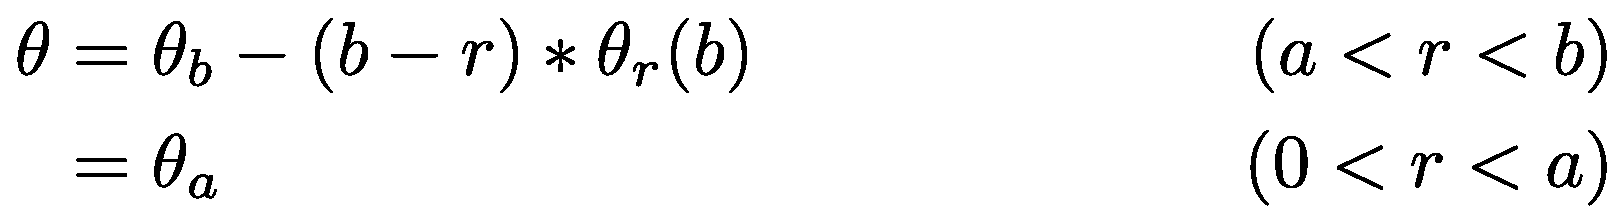
\includegraphics[width=7.0in]{psi-extension-1}
     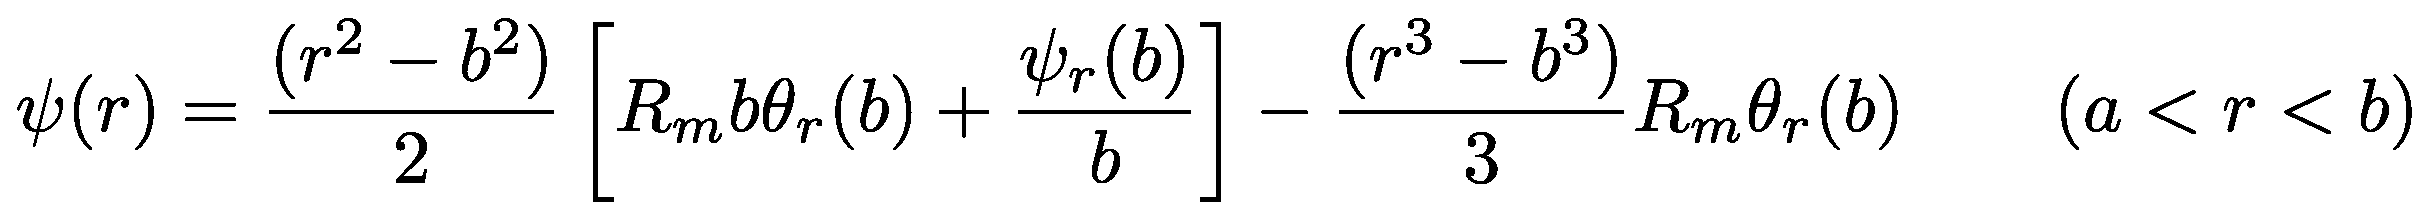
\includegraphics[width=7.0in]{psi-extension-2}
     \caption{Courtesy of Rees Jones}
 \end{figure}
 

\subsubsection{Finding $a$}
In a number of calculations we need $a$, though our grid only extends to $b$. To find $a$ we extrapolate using the condition for marginal equilibrium:
\begin{eqnarray}
f(r, z) &\equiv& \mathbf{q} \cdot \nabla \theta
\end{eqnarray}
to be finished

\subsection{Summary Diagram}

\begin{figure}[ht!]
    \centering
    \includegraphics[width=7.0in]{axiBoundaryConditions}
     \label{fig:boundary-conditions}
     \caption{Summary of equations and boundary conditions}
 \end{figure}
 

\subsection{Discretization}



In axisymmetry, the governing equations are (from section~\ref{sec:some-theory})
\begin{eqnarray}
\psi_r / r^2 - \psi_{zz}/r - \psi_{rr}/r &=& R_m \theta_r \\
r \theta_t + \psi_r \theta_z - \psi_z \theta_r - r \theta_z &=& (r \theta_r)_r + r \theta_{zz} \\
\mathbf{u} &=& \left(-\psi_z / r, \psi_r / r \right)
\end{eqnarray}

The discretization of each term is:
\begin{eqnarray}
\theta_r &\approx& \frac{\theta_{i+1, j} - \theta_{i-1, j}}{2 \Delta r} \\
\theta_z &\approx& \frac{\theta_{i, j+1} - \theta_{i, j-1}}{2 \Delta z} \\
\psi_r &\approx& \frac{\psi_{i+1, j} - \psi_{i-1, j}}{2 \Delta r} \\
\theta_{zz} &\approx& \frac{\theta_{i, j+1} + \theta_{i, j-1} - 2 \theta_{i,j}}{(\Delta z)^2}  \\
\psi_{zz} &\approx& \frac{\psi_{i, j+1} + \psi_{i, j-1} - 2 \psi_{i,j}}{(\Delta z)^2} \\
\psi_{rr} &\approx& \frac{\psi_{i+1, j} + \psi_{i-1, j} - 2 \psi_{i,j}}{(\Delta r)^2} \\
(r \theta_r)_r &\approx& \frac{(r \theta_r)_{i+1/2, j} - (r \theta_r)_{i-1/2,j}}{ \Delta r} \\
&\approx&  \frac{1}{(\Delta r)^2} \left[ r_{i+1/2} \left( \theta_{i+1, j} - \theta_{i, j} \right) - r_{i-1/2} \left( \theta_{i, j} - \theta_{i-1, j} \right)\right]
\end{eqnarray}
So the first equation becomes
\begin{eqnarray}
&&\psi_{i,j} = \frac{r_i}{2 \left( \frac{1}{(\Delta z)^2} + \frac{1}{(\Delta r)^2}\right)} \left[ f_{i,j} + \left(\frac{1}{r_i (\Delta r)^2} - \frac{1}{2 r_i^2 \Delta r} \right) \psi_{i+1, j} +                            \left(\frac{1}{r_i (\Delta r)^2} + \frac{1}{2 r_i^2 \Delta r} \right) \psi_{i-1, j} +               \frac{1}{r_i (\Delta z)^2} \left(\psi_{i,j-1} + \psi_{i, j+1} \right)                         \right] \\
&&\text{where} f_{i,j} = R_m  \frac{\theta_{i+1, j} - \theta_{i-1, j}}{2 \Delta r}
\end{eqnarray}
This will be solved using SOR:
\begin{multline}
  \psi^n_{i,j} = (1-w) \psi_{i,j}^{n-\frac{1}{2}} + w \frac{r_i}{2 \left( \frac{1}{(\Delta z)^2} + \frac{1}{(\Delta r)^2}\right)} \left[ f_{i,j} + \left(\frac{1}{r_i (\Delta r)^2} - \frac{1}{2 r_i^2 \Delta r} \right) \psi_{i+1, j} +                            \left(\frac{1}{r_i (\Delta r)^2} + \frac{1}{2 r_i^2 \Delta r} \right) \psi_{i-1, j} \right.   \\
  +   \left. \frac{1}{r_i (\Delta z)^2} \left(\psi_{i,j-1} + \psi_{i, j+1} \right)                         \right] 
\end{multline}
The heat equation is dealt with by an ADI scheme. First we discretize temporally
\begin{eqnarray}
r \frac{\theta^{n+1/2} - \theta^n}{\Delta t / 2} = \frac{1}{2} \left(              \partial_r (r \partial_r) + r \partial_{zz} + \psi_z \partial_r - \psi_r \partial_z + r \partial_z            \right) \left( \theta^{n+1/2} + \theta^n \right)
\end{eqnarray} 
Splitting this into two equations, each implicit in one direction and explicit in the other, gives
\begin{eqnarray}
r \frac{\theta^{n+1/4} - \theta^n}{\Delta t / 4} &=& \left(  r \partial_{zz} -  \psi_r^n \partial_z + r \partial_z   \right) \theta^{n+1/4} + \left(  \partial_r (r \partial_r) +   \psi_z^n \partial_r    \right) \theta^{n}  \\
r \frac{\theta^{n+1/2} - \theta^{n+1/4}}{\Delta t / 4} &=&\left(  r \partial_{zz} -  \psi_r^n \partial_z + r \partial_z   \right) \theta^{n+1/4}   +   \left(  \partial_r (r \partial_r) +   \psi_z^{n+1/4} \partial_r    \right) \theta^{n+1/2}        
\end{eqnarray}
Re-arranging (and dropping the frame advection term for now):
\begin{eqnarray}
\left( 1 - \frac{\Delta t}{4} \partial_{zz} + \frac{\Delta t \psi_r}{4 r} \partial_z \right) \theta^{n+1/4} &=& \left(1 + \frac{\Delta t}{4 r} \partial_r (r \partial_r) + \frac{\Delta t \psi_z}{4 r} \partial_r \right) \theta^n \\
\left(1 - \frac{\Delta t}{4 r} \partial_r (r \partial_r) - \frac{\Delta t \psi_z}{4 r} \partial_r \right) \theta^{n+1/2} &=& \left( 1 + \frac{\Delta t}{4} \partial_{zz} - \frac{\Delta t \psi_r}{4 r} \partial_z \right) \theta^{n+1/4} 
\end{eqnarray}
and then discretising spatially
\newpage
\begin{multline}
 1 - \frac{\Delta t}{4 (\Delta z)^2} \left(\theta^{n+1/4}_{i, j+1} + \theta^{n+1/4}_{i, j-1} - 2 \theta^{n+1/4}_{i,j}\right) + \frac{\Delta t \psi_r}{8 r \Delta z} \left(\theta^{n+1/4}_{i,j+1} - \theta^{n+1/4}_{i, j-1} \right) = \\ 1 + \frac{\Delta t}{4 r (\Delta r)^2} \left(r_{i+1/2} \theta^n_{i+1, j} + r_{i-1/2} \theta^n_{i-1,j} - (r_{i+1/2} + r_{i-1/2}) \theta^n_{i,j} \right) + \frac{\Delta t \psi_z}{8 r \Delta r} \left( \theta^n_{i+1,j} - \theta^n_{i-1,j} \right)
\end{multline}
\begin{multline}
 1 - \frac{\Delta t}{4 r (\Delta r)^2} \left(r_{i+1/2} \theta^{n+1/2}_{i+1, j} +  r_{i-1/2} \theta^{n+1/2}_{i-1,j} - (r_{i+1/2} + r_{i-1/2}) \theta^{n+1/2}_{i,j} \right) - \frac{\Delta t \psi_z}{8 r \Delta r} \left( \theta^{n+1/2}_{i+1,j} - \theta^{n+1/2}_{i-1,j} \right)= \\ 1 + \frac{\Delta t}{4 (\Delta z)^2} \left(\theta^{n+1/4}_{i, j+1} + \theta^{n+1/4}_{i, j-1} - 2 \theta^{n+1/4}_{i,j}\right) - \frac{\Delta t \psi_r}{8 r \Delta z} \left(\theta^{n+1/4}_{i,j+1} - \theta^{n+1/4}_{i, j-1} \right)
\end{multline}

Defining
\begin{eqnarray}
H_r &=& \frac{\Delta t}{4 r (\Delta r)^2} \hspace{10ex} H_z = \frac{\Delta t}{4 (\Delta z)^2} \\
P_{i,j}^n &=& \frac{(\psi_z)_{i,j}^n  \Delta t }{8 r \Delta r} \hspace{10ex} Q_{i,j}^n = \frac{ (  (\psi_r)_{i,j}^n) \Delta t}{8 r \Delta z}
\end{eqnarray}

this becomes

\begin{multline}
 \theta^{n+1/4}_{i,j} - H_z \left(\theta^{n+1/4}_{i, j+1} + \theta^{n+1/4}_{i, j-1} - 2 \theta^{n+1/4}_{i,j}\right) + Q_{i,j}^n \left(\theta^{n+1/4}_{i,j+1} - \theta^{n+1/4}_{i, j-1} \right) = \\ \theta^{n+1/2}_{i,j} + H_r\left(r_{i+1/2} \theta^n_{i+1, j} + r_{i-1/2} \theta^n_{i-1,j} - (r_{i+1/2} + r_{i-1/2}) \theta^n_{i,j} \right) + P_{i,j}^n \left( \theta^n_{i+1,j} - \theta^n_{i-1,j} \right)
\end{multline}
\begin{multline}
 \theta^{n+1/2}_{i,j} - H_r \left(r_{i+1/2} \theta^{n+1/2}_{i+1, j} +  r_{i-1/2} \theta^{n+1/2}_{i-1,j} - (r_{i+1/2} + r_{i-1/2}) \theta^{n+1/2}_{i,j} \right) - P_{i,j}^n \left( \theta^{n+1/2}_{i+1,j} - \theta^{n+1/2}_{i-1,j} \right)= \\ \theta^{n+1/4}_{i,j} + H_z \left(\theta^{n+1/4}_{i, j+1} + \theta^{n+1/4}_{i, j-1} - 2 \theta^{n+1/4}_{i,j}\right) - Q_{i,j}^n \left(\theta^{n+1/4}_{i,j+1} - \theta^{n+1/4}_{i, j-1} \right)
\end{multline}

and then collecting terms we finally arrive at 


\begin{eqnarray}
  ( - Q_{i,j}^n - H_z) \theta_{i,j-1}^{n+1/4}                           +    (1 + 2 H_z) \theta_{i,j}^{n+1/4}                         + ( Q_{i,j}^n - H_z ) \theta_{i, j+1}^{n+1/4}  = \\ 
  (-P_{i,j}^{n} + H_r r_{i-1/2}) \theta_{i-1,j}^{n}                        +       (1 - H_r (r_{i+1/2} + r_{i-1/2}) ) \theta_{i,j}^{n}      +  (P_{i,j}^{n} + H_r r_{i+1/2}) \theta_{i+1,j}^{n}            
\end{eqnarray}
and
\begin{eqnarray}
 (P_{i,j}^{n} - H_r r_{i-1/2}) \theta_{i-1,j}^{n+1/2}  		+		 (1 +  H_r (r_{i+1/2} + r_{i-1/2}) ) \theta_{i,j}^{n+1/2} +                                                           +  ( - P_{i,j}^{n} - H_r r_{i+1/2}) \theta_{i+1,j}^{n+1/2} = \\
(Q_{i,j}^{n} + H_z) \theta_{i,j-1}^{n+1/4} 		+			 (1 - 2 H_z) \theta_{i,j}^{n+1/4} 					+  (- Q_{i,j}^{n} + H_z ) \theta_{i, j+1}^{n+1/4} 
\end{eqnarray}
where

Written as matrices for an arbitrary timestep $\delta$, this looks like
\begin{eqnarray}
\left( \begin{array}{c c c c c c c}
1				&0					&0					&\hdots					&0						&0\\	
P^{n}_{2,j} - H_r r_{1.5}&1+ H_r (r_{1.5} + r_{2.5})	&-P^{n}_{2,j} - H_r r_{2.5} 	& \hdots 					& \vdots					&\vdots\\
\vdots 			& \ddots 				& \ddots 				& \ddots 					& 0						&0\\		
0 				& \hdots 				&0	 				&P^{n}_{N_r-1,j} -  H_r r_{N_r-3/2} 	&1+ H_r (r_{N_r-3/2} + r_{N_r-1/2})	& -P^{n}_{N_r-1,j} - H_r r_{N_r-1/2} \\
0 				& \hdots 				&0	 				& \hdots					&0						& 1  
\end{array} \right) \cdot \\
\left( \begin{array}{c}
\theta^{n+\delta/2}_{1,j}  \\
\theta^{n+\delta/2}_{2,j} \\
\vdots \\
\theta^{n+\delta/2}_{N_r,j} \end{array} \right)
=
\left( \begin{array}{c}
 \theta^n_{1,j} \\
(1-2 H_z r_{2,j}) \theta^n_{2,j} + (Q^n_{2,j} + H_z r_{2,j}  ) \theta^n_{2, j-1} + (-Q^n_{2,j} + H_z r_{2,j}  ) \theta^n_{2, j+1}   \\
(1-2 H_z r_{3,j}) \theta^n_{3,j} + (Q^n_{3,j} + H_z r_{3,j} ) \theta^n_{3, j-1} + (-Q^n_{3,j} + H_z r_{3,j}  ) \theta^n_{3, j+1}   \\\\
\vdots \\
\theta^n_{N_r,j} \end{array} \right) \hspace{15ex}
\end{eqnarray}
for $j = 2...(N_z-1)$, and then


\begin{eqnarray}
\left( \begin{array}{c c c c c c c}
1				&0					&0					&\hdots					&0			&0\\	
Q^{n}_{i,2} - H_z r_i	&1+2 H_z r_i				&-Q^{n}_{i,2} - H_z r_i 		& \hdots 					& \vdots		&\vdots\\
\vdots 			& \ddots 				& \ddots 				& \ddots 					& 0			&0\\		
0 				& \hdots 				&0	 				&Q^{n}_{i, N_z-1} - H_z r_{i} 		&1+2 H_z r_i 	& -Q^{n}_{i, N_z-1} - H_z r_{i} \\
0 				& \hdots 				&0	 				&\hdots					& 0			& 1  
\end{array} \right) \cdot \\
\left( \begin{array}{c}
\theta^{n+\delta}_{i,1}  \\
\theta^{n+\delta}_{i,2} \\
\vdots \\
\theta^{n+\delta}_{i,N_z} \end{array} \right)
=
\left( \begin{array}{c}
 \theta^{n+\delta/2}_{i,1} \\
(1- H_r (r_{i+1/2} + r_{i-1/2}) ) \theta^{n+\delta/2}_{i,2} +         (P^n_{i,2} + H_r r_{i-1/2} ) \theta^{n+\delta/2}_{i-1, 2} +           (-P^{n+\delta/2}_{i,2} +H_r r_{i+1/2} ) \theta^{n+\delta/2}_{i+1, 2}   \\
(1- H_r (r_{i+1/2} + r_{i-1/2}) ) \theta^{n+\delta/2}_{i,3} +         (P^n_{i,3} + H_r r_{i-1/2}) \theta^{n+\delta/2}_{i-1, 3} +           (-P^{n+\delta/2}_{i,3} + H_r r_{i+1/2} ) \theta^{n+\delta/2}_{i+1, 3}   \\
\vdots \\
\theta^{n+\delta/2}_{i,N_z} \end{array} \right) \hspace{15ex}
\end{eqnarray}
for $i= 1... (N_r - 1)$

To test the code, we will look at the problem described in Nield and Bejan p.118. Namely (with $x$ changed to $z$ for consistency)
\begin{eqnarray}
\frac{\partial}{\partial r} \left( \frac{1}{r} \frac{\partial \psi}{\partial r} \right) &=& \frac{g \beta K}{\nu} \frac{\partial T}{\partial r} \\
\frac{\partial \psi}{\partial r} \frac{\partial T}{\partial z} - \frac{\partial \psi}{\partial z} \frac{\partial T}{\partial r} &=& \alpha_m \frac{\partial}{\partial r} \left(r \frac{\partial T}{\partial r} \right)
\end{eqnarray}
we set $\alpha_m = 1$, let $R_m =  \frac{g \beta K}{\nu}$ and include the general axisymmetric terms that have been omitted:
\begin{eqnarray}
\frac{\partial}{\partial r} \left( \frac{1}{r} \frac{\partial \psi}{\partial r} \right) + \frac{1}{r}\frac{\partial^2 \psi}{\partial z^2} &=& R_m \frac{\partial T}{\partial r} \\
r \frac{\partial T}{\partial t} + \frac{\partial \psi}{\partial r} \frac{\partial T}{\partial z} - \frac{\partial \psi}{\partial z} \frac{\partial T}{\partial r} - r \frac{\partial T}{\partial z} &=& \frac{\partial}{\partial r} \left(r \frac{\partial T}{\partial r} \right) + r \frac{\partial^2 T}{\partial z^2}
\end{eqnarray}
Considering the cylindrical ($\lambda = 1$) case, with the constant $A=1$ for simplicity, the boundary conditions we will implement are
\begin{eqnarray}
T(r=R, z) = T_\infty + z \hspace{5ex} u_r(r=R) = 0 \\
T(\infty) = T_\infty \hspace{8ex} u_z(r=\infty) = 0
\end{eqnarray}
Where $R$ is the radius of the cylinder. For finite derivatives of $\psi_r$, the condition $u_z(r=\infty) = 0$ is automatically satisfied by the choice of streamfunction.

Similarity variables are defined as
\begin{eqnarray}
\eta &=& Ra_z \left( \frac{r}{z} \right)^2 \\
\psi &=& z f(\eta) \label{eq:psi-analytic-axisymm} \\
T &=& T_\infty + (T_w(z) - T_\infty) \theta(\eta) = T_\infty + z \theta(\eta)
\end{eqnarray}
and, as $Ra_z = R_m z^2$, the equation for $\eta$ simplifies to
\begin{eqnarray}
\eta &=& R_m r^2
\end{eqnarray}
So in our similarity variables, the surface of the cylinder is at $\eta = a_{nc} = R_m R^2$. Note that, from our definition of the stream function,
\begin{eqnarray}
u_r = - \frac{f(\eta)}{r} \hspace{10ex} u_z = R_m z \theta(\eta)
\end{eqnarray}

$f$ and $\theta$ are then the solutions to the equations
\begin{eqnarray}
2f' = \theta \\
2 \eta \theta'' + (2+f) \theta' - f' \theta = 0
\end{eqnarray}
which are solved using ode45 to give an `analytical' solution which the code can be tested against.

We will use $a_{nc} = 0.1$ and $R_m = 10$, and we observe that the code correctly reproduces the analytic steady state solution.

\section{Preliminary results}
Using a straight chimney, with width determined by previous studies, and an approximate concentration profile
\begin{eqnarray}
C(z) = -1 + \frac{z}{2 H}
\end{eqnarray}
we have been able to reach a steady state that exhibits the same features as previous investigations.

The next step is to determine the chimney width, $a$, based on the values of the temperature and fluid velocity at $r=b$.

\begin{figure}[ht!]
    \centering
    \includegraphics[width=5.0in]{mushyLayerStreamlinesExample}
     \label{fig:streamlines}
     \caption{Example convection cell}
 \end{figure}
 
 \begin{figure}[ht!]
    \centering
    \includegraphics[width=5.0in]{mushyLayerThetaContourExample}
     \label{fig:contours}
     \caption{Example heat profile}
 \end{figure}


\end{document}